\begin{center}
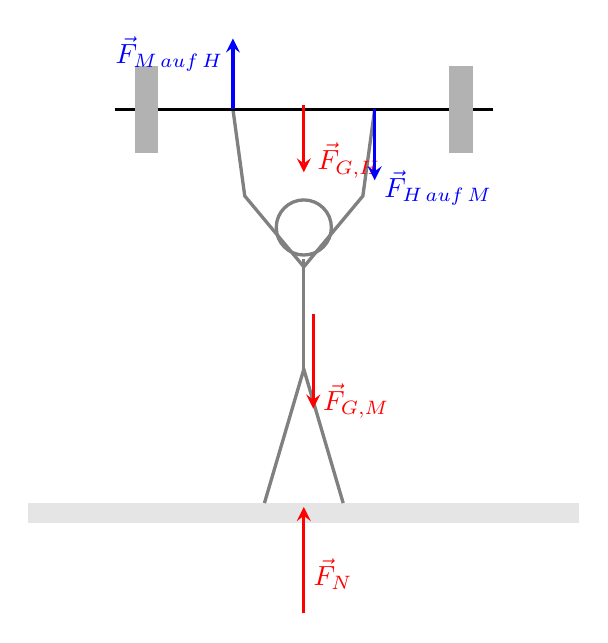
\begin{tikzpicture}[>=stealth]
 \draw (-3.5,0) -- (3.5,0);
 \fill[gray!20] (-3.5,0) rectangle (3.5,-0.25);
 \draw[gray, very thick] (-0.5,0) -- (0,1.7) -- (0.5,0);
 \draw[gray, very thick] (0,1.7) -- (0,3.1);
 \draw[gray, very thick] (0,3.5) circle (0.35);
 \draw[gray, very thick] (0,3.0) -- (-0.75,3.9) -- (-0.9,5);
 \draw[gray, very thick] (0,3.0) -- (0.75,3.9) -- (0.9,5);
 \draw[very thick] (-2.4,5) -- (2.4,5);
 \fill[gray!60] (-2.15,4.45) rectangle (-1.85,5.55);
 \fill[gray!60] (1.85,4.45) rectangle (2.15,5.55);
 \draw[->, very thick, red] (0,5.05) -- (0,4.2);
 \node[red, right] at (0.05,4.35) {$\vec F_\text{G,H}$};
 \draw[->, very thick, red] (0.12,2.4) -- (0.12,1.2);
 \node[red, right] at (0.12,1.3) {$\vec F_\text{G,M}$};
 \draw[->, very thick, red] (0,-1.4) -- (0,-0.05);
 \node[red, right] at (0,-0.9) {$\vec F_\text{N}$};
 \draw[->, very thick, blue] (-0.9,5) -- (-0.9,5.9);
 \node[blue, left] at (-0.9,5.7) {$\vec F_\text{M\,auf\,H}$};
 \draw[->, very thick, blue] (0.9,5) -- (0.9,4.1);
 \node[blue, right] at (0.9,4.0) {$\vec F_\text{H\,auf\,M}$};
\end{tikzpicture}
\end{center}
(Die Kräfte der Hände sind für jede Hand vorhanden; der Übersicht halber ist jede Art nur bei einer Hand gezeichnet.)

\emph{Äussere Kräfte} (rot, sie stammen von Körpern ausserhalb des Systems):
\begin{itemize}
\item Gewichtskraft der Hantel $\vec F_\text{G,H}$ (die Erde zieht die Hantel an). Reaktionspartner: Die Hantel zieht die Erde an.
\item Gewichtskraft des Gewichthebers $\vec F_\text{G,M}$. Reaktionspartner: Der Gewichtheber zieht die Erde an.
\item Normalkraft $\vec F_\text{N}$ des Bodens auf die Füsse. Reaktionspartner: Die Füsse drücken mit gleich grosser Kraft auf den Boden.
\end{itemize}

\emph{Innere Kräfte} (blau, beide Partner gehören zum System):
\begin{itemize}
\item Die Hände stossen die Hantel nach oben, $\vec F_\text{M\,auf\,H}$. Reaktionspartner: Die Hantel drückt die Hände nach unten, $\vec F_\text{H\,auf\,M}$.
\item Ebenso alle Kräfte zwischen Körperteilen des Gewichthebers (Muskeln, Gelenke).
\end{itemize}

Im Gleichgewicht gilt für die Hantel $F_\text{M\,auf\,H} = F_\text{G,H}$ und für das ganze System $F_\text{N} = F_\text{G,H}+F_\text{G,M}$.

\emph{Beim Stemmen} bleiben die Gewichtskräfte gleich. Es ändern sich die Kraft zwischen Händen und Hantel und damit auch die Normalkraft des Bodens (und die Reaktionskräfte dazu): Solange die Hantel nach oben beschleunigt wird, sind sie grösser, beim Abbremsen kleiner als im Gleichgewicht.
